% MI4MedFM 2026 LNCS proceedings submission draft.
% Compile from the paper/ directory after placing Springer llncs.cls there
% or installing it in the local TeX path.
\documentclass[runningheads]{llncs}

\usepackage[T1]{fontenc}
\usepackage{graphicx}
\usepackage{booktabs}
\usepackage{amsmath}
\usepackage{url}

\graphicspath{{assets/}}

\begin{document}

\title{Counterfactual Activation Patching Reveals Context-Mediated Boundary Failures in MedSAM}
\titlerunning{Counterfactual Activation Patching in MedSAM}

\author{Anonymous MI4MedFM Submission}
\authorrunning{Anonymous}
\institute{Anonymous Institution}

\maketitle

\begin{abstract}
Medical segmentation foundation models can fail when pathology obscures anatomical boundaries, but output masks alone do not identify which internal computations mediate the failure. We study this question in MedSAM on pleural-effusion chest radiographs, where the lower lung boundary is often weak or hidden. For each diseased image, we pair the original radiograph with a pseudo-healthy counterfactual and use the pair as a causal probe of MedSAM's image encoder. We run MedSAM with the same lung bounding-box prompt on original and counterfactual images, patch internal activations between paired forward passes, and test matched, reverse, non-matched, boundary-band, and background/context interventions. On 50 NIH ChestX-ray14 pleural-effusion cases with CheXMask silver lung masks, CF-Seg counterfactuals improve MedSAM Dice from 0.677 to 0.831, Boundary F1 from 0.139 to 0.207, and HD95 from 131.0 to 93.1 pixels. Matched whole-map activation patching reproduces the counterfactual improvement, reverse patching returns to original-like behavior, and non-matched donor patching performs substantially worse. Region controls show that background/context activations carry more corrective signal than a thin boundary band, suggesting that the observed boundary failure is mediated by broader patient-specific context and shape representations. A diffusion counterfactual run on the same 50 cases reproduces the matched-versus-non-matched causal pattern, although it is weaker than CF-Seg for Boundary F1. These results position counterfactual images as mechanistic probes for medical foundation models rather than only as preprocessing inputs for better masks.

\keywords{Mechanistic interpretability \and Medical foundation models \and MedSAM \and Activation patching \and Counterfactual imaging \and Chest radiography}
\end{abstract}

\section{Introduction}

Promptable segmentation foundation models have made it practical to segment many medical structures with a common interface. MedSAM adapts the Segment Anything Model (SAM) to medical images and accepts spatial prompts such as bounding boxes to produce target masks across modalities \cite{kirillov2023segment,ma2024medsam}. This flexibility is useful in clinical workflows, but it does not remove a familiar failure mode of medical segmentation: when disease changes, occludes, or weakens an anatomical boundary, the predicted mask may fail in ways that are difficult to diagnose from the final output alone.

Pleural effusion in chest radiography is a concrete example. Fluid and opacity near the costophrenic angle can obscure the lower lung contour, so a lung segmentor may under-segment the diseased hemithorax or place a boundary at the edge of the opacity rather than the anatomical lung extent. A mask-level evaluation can show that Dice, Boundary F1, or HD95 worsened, but it does not say whether the failure is caused by missing local edge evidence, a changed global shape representation, prompt sensitivity, or later mask-decoder behavior.

Counterfactual image generation creates a useful experimental handle on this problem. CF-Seg showed that pseudo-healthy chest X-rays can improve lung segmentation in pleural-effusion cases \cite{mehta2025cfseg}. That result is important, but it treats the counterfactual primarily as an output-improvement tool: generate a healthier-looking image, segment that image, and use the improved mask. Here we ask a mechanistic question instead. If a patient-matched pseudo-healthy counterfactual restores the lung boundary, which internal MedSAM activations causally carry that restoration?

We propose \emph{counterfactual activation patching} for medical segmentation foundation models. Given an original diseased image and a patient-matched pseudo-healthy counterfactual, we run both inputs through MedSAM with the same bounding-box prompt. We then replace selected image-encoder activations in one forward pass with activations from the other. If patching counterfactual activations into the original-image run restores segmentation quality, and patching original activations into the counterfactual run removes that restoration, the intervention gives causal evidence that those representations mediate the output behavior.

Our study focuses on an intentionally compact but controlled 50-case NIH ChestX-ray14 pleural-effusion subset with CheXMask silver lung masks \cite{wang2017chestxray8,gaggion2024chexmask,gaggion2025chexmask,goldberger2000physionet}. The results support three claims. First, patient-matched pseudo-healthy counterfactuals substantially improve MedSAM lung segmentation under pleural effusion. Second, the improvement is causally mediated by internal image-encoder representations: matched whole-map activation patching reproduces the counterfactual result, while reverse and non-matched controls do not. Third, the causal signal is not confined to a thin anatomical boundary band. Background/context patching is stronger than boundary-band patching across CF-Seg and diffusion counterfactuals, suggesting a context-mediated boundary-failure mechanism.

\section{Related Work}

\paragraph{Medical segmentation foundation models.}
SAM introduced promptable segmentation at scale using a large image encoder, prompt encoder, and mask decoder \cite{kirillov2023segment}. Several studies have observed that direct SAM transfer to medical images is uneven because medical structures can have lower contrast, different texture statistics, and more ambiguous object definitions than natural-image objects \cite{mazurowski2023sam,huang2024sammedical}. MedSAM addresses this domain gap by adapting SAM to a large collection of medical image-mask pairs and has become a common foundation model for promptable medical segmentation \cite{ma2024medsam}. Our work does not propose another segmentor; it uses MedSAM as the target system whose internal failure mechanisms are probed.

\paragraph{Counterfactual medical image generation.}
Counterfactual radiographs are often used to ask what an image would look like if a pathology were absent, milder, or more severe. CF-Seg is the closest prior work to our experimental setting: it generates pseudo-healthy chest X-rays from pleural-effusion cases and shows that the generated images can support better lung segmentation \cite{mehta2025cfseg}. Diffusion models, including latent diffusion and Stable Diffusion variants, provide another route to image editing and counterfactual synthesis \cite{rombach2022ldm,liang2023pie}. In our experiments, CF-Seg is the primary counterfactual source and a MIMIC-CXR Stable Diffusion model is used as an independent generator check. The distinction from prior counterfactual-segmentation work is the target of explanation: we use counterfactuals to intervene on MedSAM activations, not only to obtain improved masks.

\paragraph{Activation patching and causal tracing.}
Mechanistic interpretability aims to identify internal computations that causally explain model behavior. Causal mediation and activation patching methods have been widely used in language models to test whether hidden states, neurons, or attention heads mediate a behavior of interest \cite{imai2010causal,vig2020causal,meng2022rome,zhang2023activationpatching}. The basic logic is to compare a clean and corrupted run, replace a component activation from one run into the other, and measure whether the output behavior is restored or suppressed. We adapt this idea to promptable medical segmentation. Here the clean/corrupted pair is not a synthetic token corruption, but a clinically meaningful original/counterfactual image pair.

\section{Methods}

\subsection{Data and Counterfactual Sources}

We use 50 frontal NIH ChestX-ray14 images labeled with pleural effusion. The subset contains 18 unique subjects, with 32 AP and 18 PA images. Lung reference masks are obtained from CheXMask at the original ChestX-ray8 resolution and are treated as silver-standard labels rather than expert annotations. We form a single combined lung target and derive a fixed bounding-box prompt from this reference mask for each case.

The primary counterfactual source is CF-Seg, using pseudo-healthy images generated for the pleural-effusion target. The secondary source is a MIMIC-CXR-finetuned Stable Diffusion model distributed as \texttt{IrohXu/stable-diffusion-mimic-cxr-v0.1}. We use image-to-image generation with the prompt ``frontal chest x-ray of a patient with no findings,'' a negative prompt targeting pleural effusion and related artifacts, strength 0.35, guidance scale 7.5, and 40 inference steps. Generated images are resized back to the original 1024 by 1024 CXR resolution before MedSAM inference. We refer to this generator as CXR-SD.

\begin{figure}
\centering
\IfFileExists{assets/figure_qualitative_generators_nih_effusion_50_3cases.png}{%
\includegraphics[width=\textwidth]{figure_qualitative_generators_nih_effusion_50_3cases.png}%
}{%
\fbox{\parbox{0.92\textwidth}{Qualitative CXR panel omitted from the anonymous code repository because it contains patient-derived pixels. The submitted PDF includes this panel when permitted by the dataset license; it can be regenerated locally from the restored manifests.}}%
}
\caption{Three representative NIH pleural-effusion cases. Orange shows the CheXMask silver reference boundary, cyan shows the MedSAM prediction, and yellow shows the fixed prompt box. CF-Seg counterfactuals often restore lower-lung extent more clearly than CXR-SD, while CXR-SD provides an independent generator condition for testing whether the causal-patching pattern is generator-specific.}
\label{fig:qualitative}
\end{figure}

\subsection{MedSAM Inference}

For each case, we run MedSAM on the original image, the CF-Seg counterfactual, and the CXR-SD counterfactual. The same box prompt is used across all image variants for a case, controlling for prompt changes and isolating the effect of the visual input. Images are resized to 1024 by 1024 for the MedSAM image encoder, and predicted masks are thresholded at 0.5 after bilinear upsampling to the image resolution.

\subsection{Counterfactual Activation Patching}

Let $x_i$ be an original pleural-effusion image, $\tilde{x}_i$ its patient-matched pseudo-healthy counterfactual, and $b_i$ the fixed lung bounding-box prompt. MedSAM's segmentation can be written as
\begin{equation}
    \hat{y} = D(E(x), b),
\end{equation}
where $E$ is the image encoder and $D$ denotes the prompt encoder and mask decoder. For an encoder layer $\ell$, let $h_\ell(x)$ denote the activation tensor at that layer. A patching intervention replaces a spatial region $R$ of the target activation with the corresponding donor activation:
\begin{equation}
    h_\ell^{\mathrm{patch}}(u, v, c) =
    \begin{cases}
        h_\ell(x_{\mathrm{donor}})(u, v, c), & (u,v) \in R, \\
        h_\ell(x_{\mathrm{target}})(u, v, c), & (u,v) \notin R .
    \end{cases}
\end{equation}
The patched activation is then passed through the remaining MedSAM computation and decoded with the same box prompt.

We patch three image-encoder sites: block 3, block 9, and the encoder neck. We evaluate the following controls:
\begin{itemize}
    \item \textbf{Matched counterfactual-to-original}: donor $\tilde{x}_i$, target $x_i$. This is the main restoration intervention.
    \item \textbf{Reverse original-to-counterfactual}: donor $x_i$, target $\tilde{x}_i$. This tests whether diseased activations remove counterfactual restoration.
    \item \textbf{Non-matched counterfactual-to-original}: donor $\tilde{x}_j$ from another case, target $x_i$. This tests patient-specificity rather than generic healthy-image feature injection.
\end{itemize}
Spatial regions include the whole activation map, a 32-pixel anatomical boundary band around the CheXMask lung contour, the lung interior, the background outside the lung mask, and random regions matched in size to the boundary or background regions. CXR-SD controls use whole, boundary, and background regions.

\begin{figure}
\centering
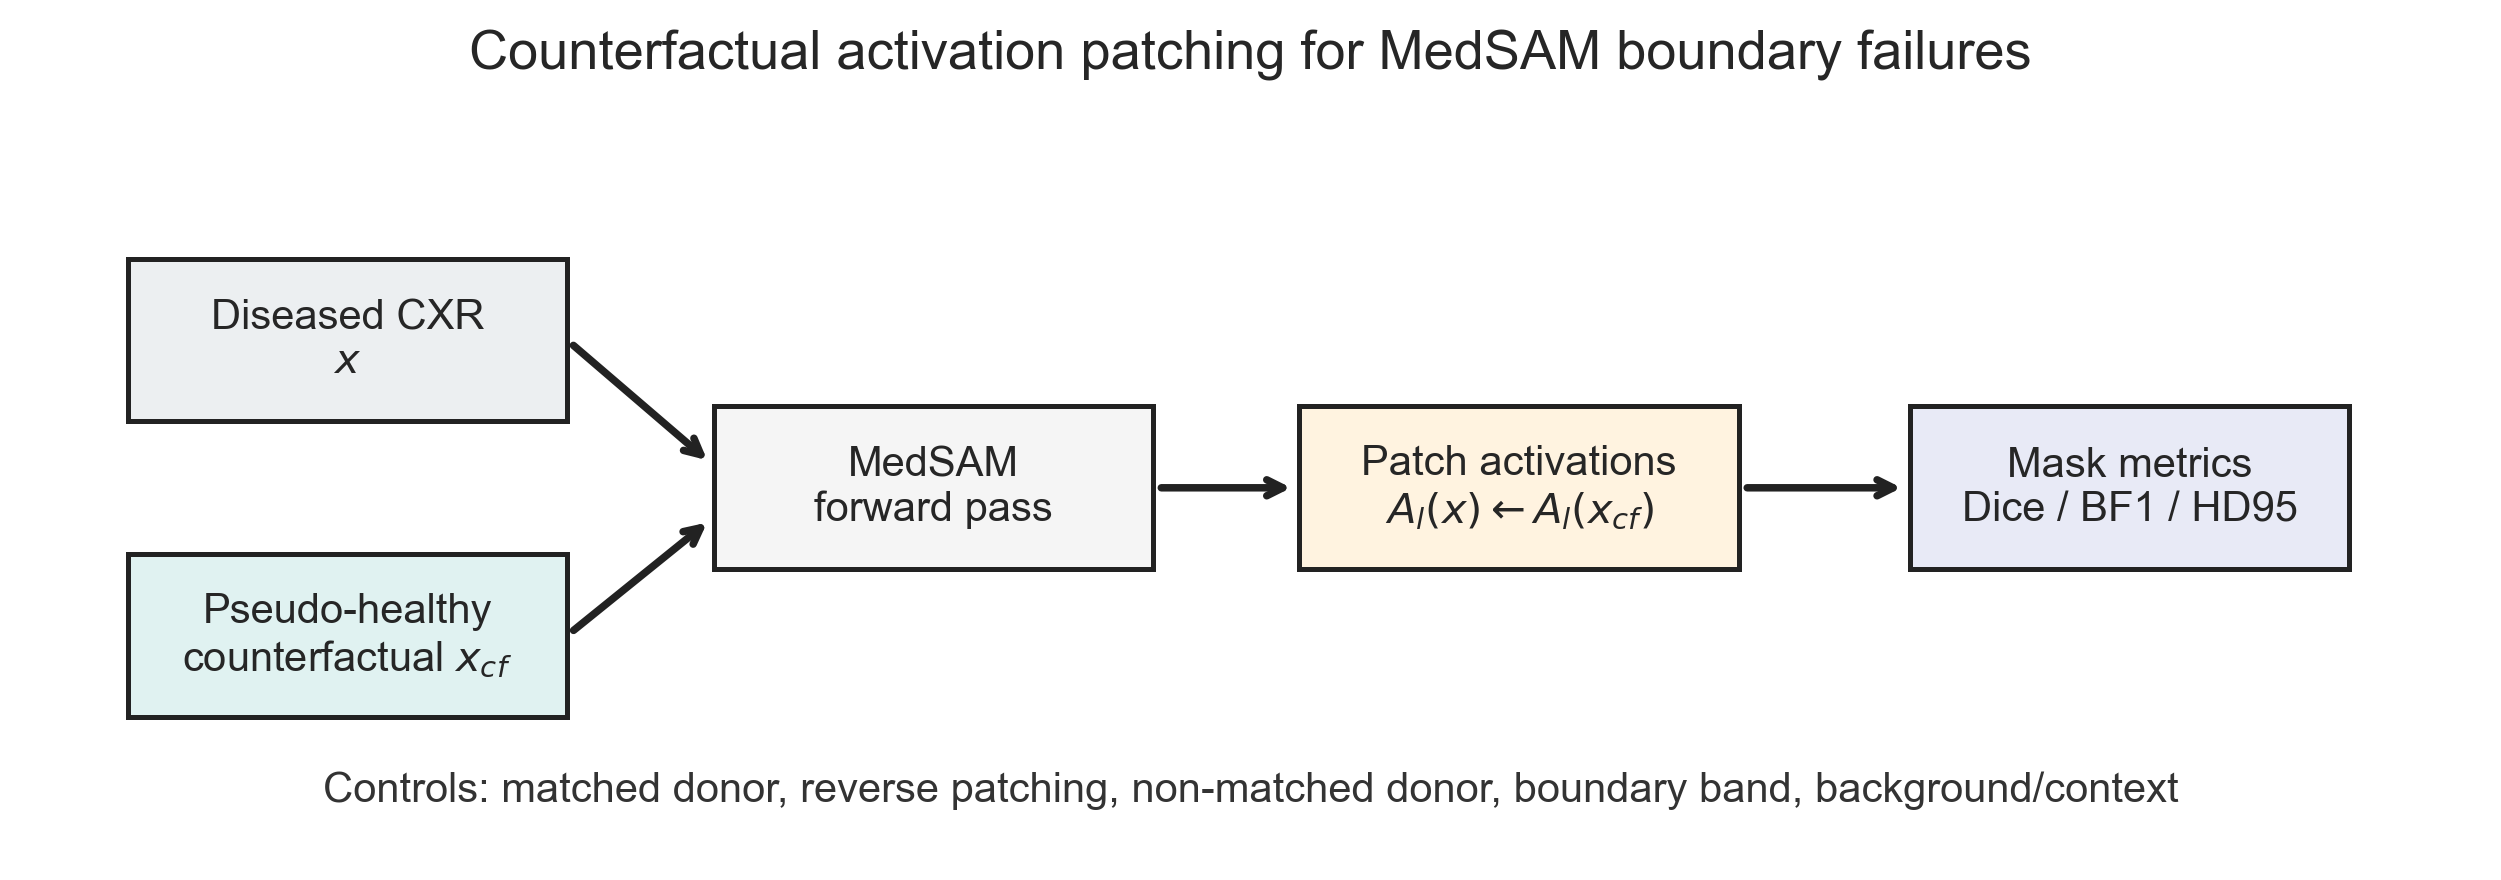
\includegraphics[width=\textwidth]{figure_method_schematic.png}
\caption{Counterfactual activation patching for MedSAM. A diseased chest radiograph and a patient-matched pseudo-healthy counterfactual are passed through MedSAM with the same lung box prompt. Activations from one run are patched into the other, and the decoded mask is evaluated against the CheXMask silver reference. Matched, reverse, non-matched, boundary-band, and background/context controls test directionality, patient-specificity, and spatial localization.}
\label{fig:method}
\end{figure}

\subsection{Metrics and Statistical Tests}

We evaluate predicted masks against CheXMask lung masks using Dice, IoU, Boundary F1 with a 3-pixel tolerance, HD95 in pixels, and signed area error relative to the reference mask, combining overlap and boundary-aware metrics in line with problem-specific image-analysis validation recommendations \cite{maierhein2024metrics}. We report paired case-level comparisons using 10,000 paired bootstrap resamples of the mean difference and two-sided Wilcoxon signed-rank tests. Because CheXMask masks are algorithmic silver references, all clinical conclusions are framed as mechanistic evidence rather than deployment-ready segmentation validation.

\section{Experiments, Results, and Analysis}

\subsection{Counterfactual Images Improve MedSAM Segmentation}

Table~\ref{tab:generator_metrics} compares MedSAM predictions on original diseased images, CF-Seg pseudo-healthy counterfactuals, and CXR-SD counterfactuals. CF-Seg provides the strongest segmentation improvement, increasing Dice from 0.677 to 0.831 and Boundary F1 from 0.139 to 0.207 while reducing HD95 from 131.0 to 93.1 pixels. The improvement is statistically robust for Dice, Boundary F1, and HD95 (Table~\ref{tab:bootstrap}). CXR-SD also improves Dice and HD95 over original images, but its Boundary F1 change is small and not statistically reliable. We therefore treat CXR-SD as a robustness check for the counterfactual-patching mechanism, not as a stronger segmentation generator.

\begin{table}
\centering
\caption{MedSAM segmentation on original and counterfactual images. Higher is better for Dice, IoU, and Boundary F1; lower is better for HD95. Area error is signed relative to the reference area, so values closer to zero are better. CheXMask masks are silver references.}
\label{tab:generator_metrics}
\small
\begin{tabular}{lrrrrrr}
\toprule
Condition & $n$ & Dice & IoU & Boundary F1 & HD95 & Area error \\
\midrule
Original & 50 & 0.677 & 0.535 & 0.139 & 131.0 & 0.312 \\
CF-Seg & 50 & 0.831 & 0.727 & 0.207 & 93.1 & 0.186 \\
CXR-SD & 50 & 0.779 & 0.653 & 0.147 & 109.6 & 0.315 \\
\bottomrule
\end{tabular}
\end{table}

\begin{table}
\centering
\caption{Paired bootstrap and Wilcoxon tests for generator comparisons. Mean difference is candidate minus baseline; negative HD95 means improvement.}
\label{tab:bootstrap}
\scriptsize
\setlength{\tabcolsep}{3.5pt}
\begin{tabular}{llrrr}
\toprule
Comparison & Metric & Mean diff. & 95\% CI & $p$ \\
\midrule
CF-Seg vs original & Dice & 0.154 & [0.113, 0.198] & $3.61{\times}10^{-12}$ \\
CF-Seg vs original & Boundary F1 & 0.068 & [0.042, 0.095] & $2.97{\times}10^{-5}$ \\
CF-Seg vs original & HD95 & -37.87 & [-54.46, -21.57] & $4.21{\times}10^{-5}$ \\
CXR-SD vs original & Dice & 0.101 & [0.060, 0.146] & $8.78{\times}10^{-7}$ \\
CXR-SD vs original & Boundary F1 & 0.007 & [-0.009, 0.024] & 0.702 \\
CXR-SD vs original & HD95 & -21.38 & [-34.07, -9.36] & $1.15{\times}10^{-3}$ \\
CF-Seg vs CXR-SD & Dice & 0.052 & [0.033, 0.072] & $1.21{\times}10^{-6}$ \\
CF-Seg vs CXR-SD & Boundary F1 & 0.061 & [0.040, 0.082] & $1.86{\times}10^{-6}$ \\
CF-Seg vs CXR-SD & HD95 & -16.49 & [-30.81, -2.66] & $2.12{\times}10^{-2}$ \\
\bottomrule
\end{tabular}
\end{table}

\subsection{Matched Activation Patching Recovers Counterfactual Behavior}

The main mechanistic test is whether the counterfactual effect is present inside MedSAM activations. Table~\ref{tab:activation_controls} summarizes the key controls. For CF-Seg, matched whole-map patching from counterfactual to original exactly recovers the MedSAM-on-counterfactual result: Dice 0.831, Boundary F1 0.207, and HD95 93.1. Reverse whole-map patching returns the counterfactual run to original-like performance. Non-matched whole-map patching is substantially worse than matched patching, with Dice 0.672 and Boundary F1 0.057. The paired matched-versus-non-matched gap is large for Dice (+0.159, 95\% CI [0.125, 0.192], $p=4.96{\times}10^{-11}$), Boundary F1 (+0.150, 95\% CI [0.116, 0.185], $p=8.84{\times}10^{-12}$), and HD95 (-42.75 pixels, 95\% CI [-59.17, -27.69], $p=1.21{\times}10^{-6}$).

\begin{table}
\centering
\caption{Activation-patching controls averaged across block 3, block 9, and neck. Whole-map matched patching recovers counterfactual-like behavior; reverse and non-matched controls test directionality and patient-specificity.}
\label{tab:activation_controls}
\scriptsize
\setlength{\tabcolsep}{3pt}
\begin{tabular}{llrrrr}
\toprule
Generator & Condition & Dice & Boundary F1 & HD95 & Area error \\
\midrule
CF-Seg & Original & 0.677 & 0.139 & 131.0 & 0.312 \\
CF-Seg & Matched whole & 0.831 & 0.207 & 93.1 & 0.186 \\
CF-Seg & Reverse whole & 0.677 & 0.139 & 131.0 & 0.312 \\
CF-Seg & Non-matched whole & 0.672 & 0.057 & 135.9 & 0.215 \\
CF-Seg & Background/context & 0.776 & 0.210 & 100.9 & 0.185 \\
CF-Seg & Boundary band & 0.695 & 0.144 & 115.7 & 0.220 \\
\midrule
CXR-SD & Original & 0.677 & 0.139 & 131.0 & 0.312 \\
CXR-SD & Matched whole & 0.779 & 0.147 & 109.6 & 0.315 \\
CXR-SD & Reverse whole & 0.677 & 0.139 & 131.0 & 0.312 \\
CXR-SD & Non-matched whole & 0.630 & 0.058 & 139.5 & 0.249 \\
CXR-SD & Background/context & 0.739 & 0.160 & 111.8 & 0.283 \\
CXR-SD & Boundary band & 0.691 & 0.131 & 128.5 & 0.328 \\
\bottomrule
\end{tabular}
\end{table}

\begin{figure}
\centering
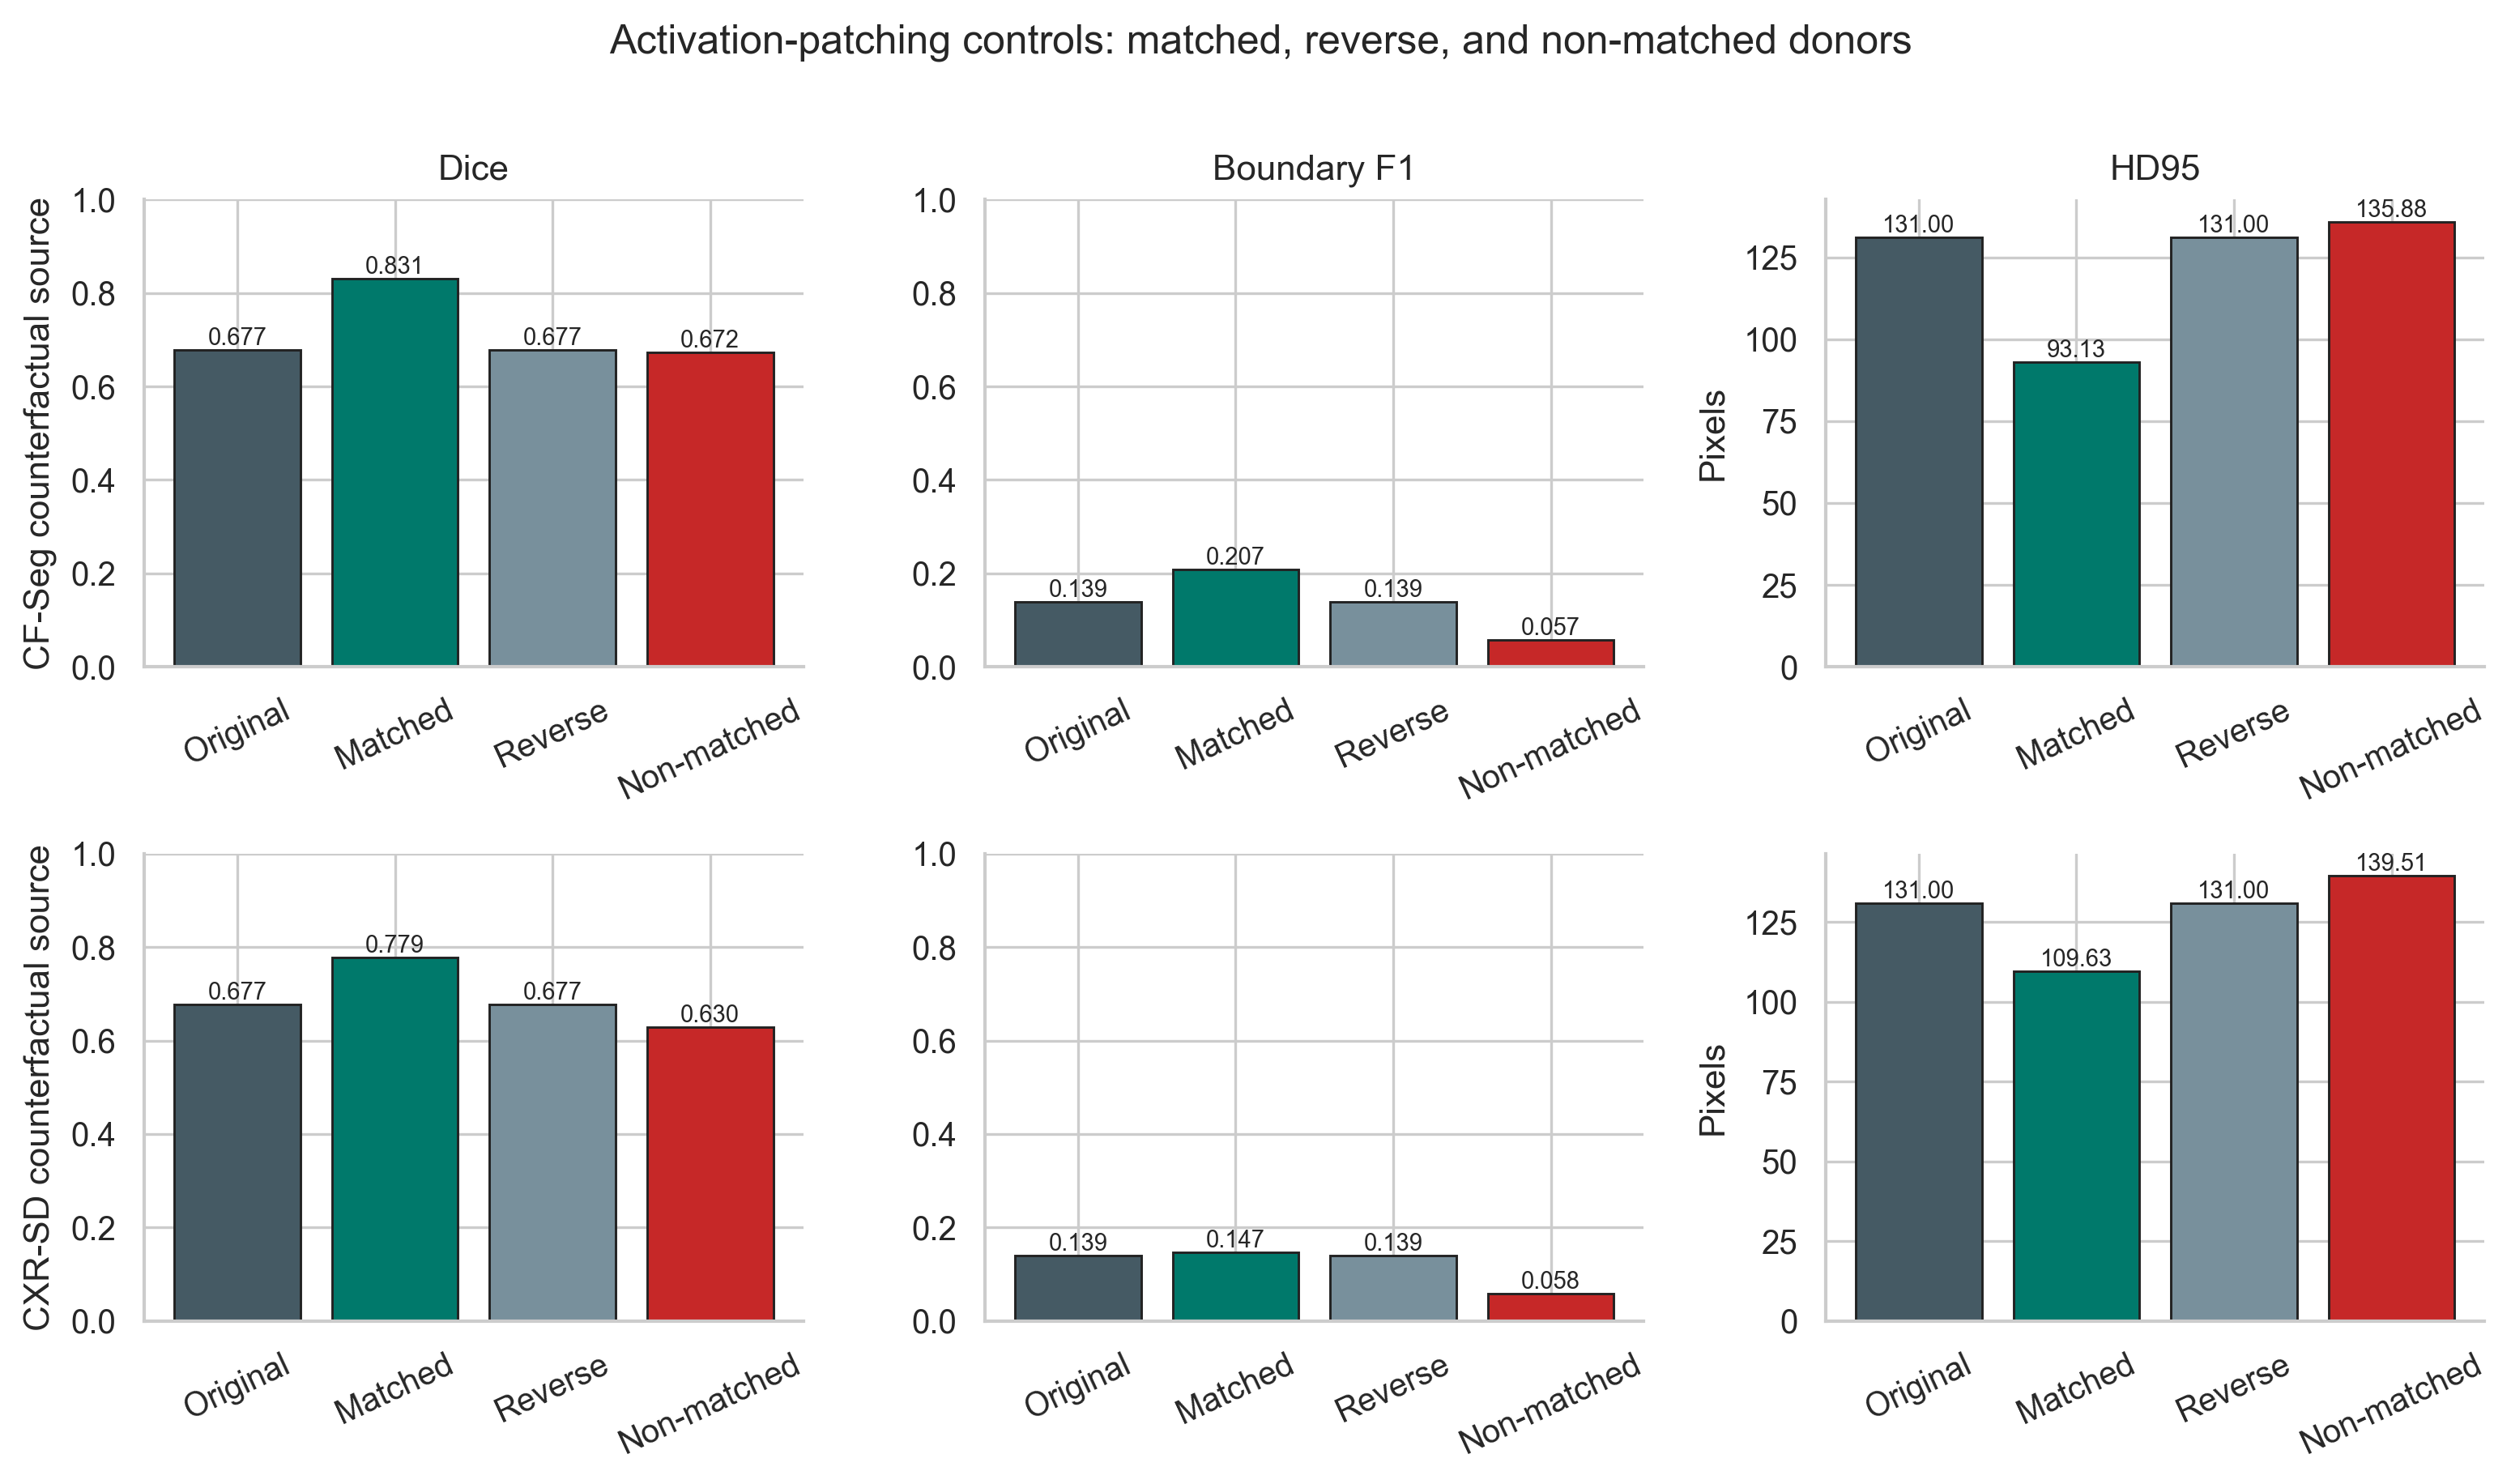
\includegraphics[width=\textwidth]{figure_activation_pairing_controls.png}
\caption{Pairing controls for CF-Seg and CXR-SD counterfactuals. Matched whole-map patching recovers counterfactual-like behavior, reverse patching returns to original-like behavior, and non-matched counterfactual donors perform substantially worse. This pattern supports patient-specific causal mediation rather than generic healthy-feature injection.}
\label{fig:pairing}
\end{figure}

The CXR-SD controls reproduce the same patient-specific pattern with a weaker generator. Matched whole-map CXR-SD patching reaches the CXR-SD counterfactual result, while non-matched CXR-SD donors perform much worse. The matched-versus-non-matched differences are statistically robust for Dice (+0.149, 95\% CI [0.113, 0.185], $p=1.62{\times}10^{-10}$), Boundary F1 (+0.088, 95\% CI [0.062, 0.116], $p=3.13{\times}10^{-10}$), and HD95 (-29.88 pixels, 95\% CI [-44.13, -15.33], $p=1.25{\times}10^{-4}$). This matters because it argues that the causal-pairing result is not an idiosyncrasy of CF-Seg.

\subsection{Boundary Failure Is Mediated by Broader Context}

The spatial controls test whether the corrective signal is concentrated in the anatomical boundary band. Contrary to a boundary-token-only explanation, background/context patching is stronger than thin boundary-band patching. For CF-Seg, background/context patching achieves Dice 0.776, Boundary F1 0.210, and HD95 100.9, compared with Dice 0.695, Boundary F1 0.144, and HD95 115.7 for boundary-band patching. The background-versus-boundary improvement is significant for Dice (+0.081, 95\% CI [0.058, 0.108], $p=5.61{\times}10^{-11}$), Boundary F1 (+0.066, 95\% CI [0.052, 0.080], $p=3.09{\times}10^{-12}$), and HD95 (-14.83 pixels, 95\% CI [-24.84, -4.46], $p=2.05{\times}10^{-3}$).

CXR-SD shows the same qualitative pattern: background/context patching outperforms boundary-band patching for Dice (+0.048, 95\% CI [0.026, 0.073], $p=9.37{\times}10^{-6}$), Boundary F1 (+0.029, 95\% CI [0.019, 0.040], $p=3.99{\times}10^{-7}$), and HD95 (-16.73 pixels, 95\% CI [-24.43, -9.48], $p=6.83{\times}10^{-5}$). The observed error is a boundary failure at the output mask, but the causal signal appears distributed across broader context and shape representations rather than isolated to a narrow edge band.

\begin{figure}
\centering
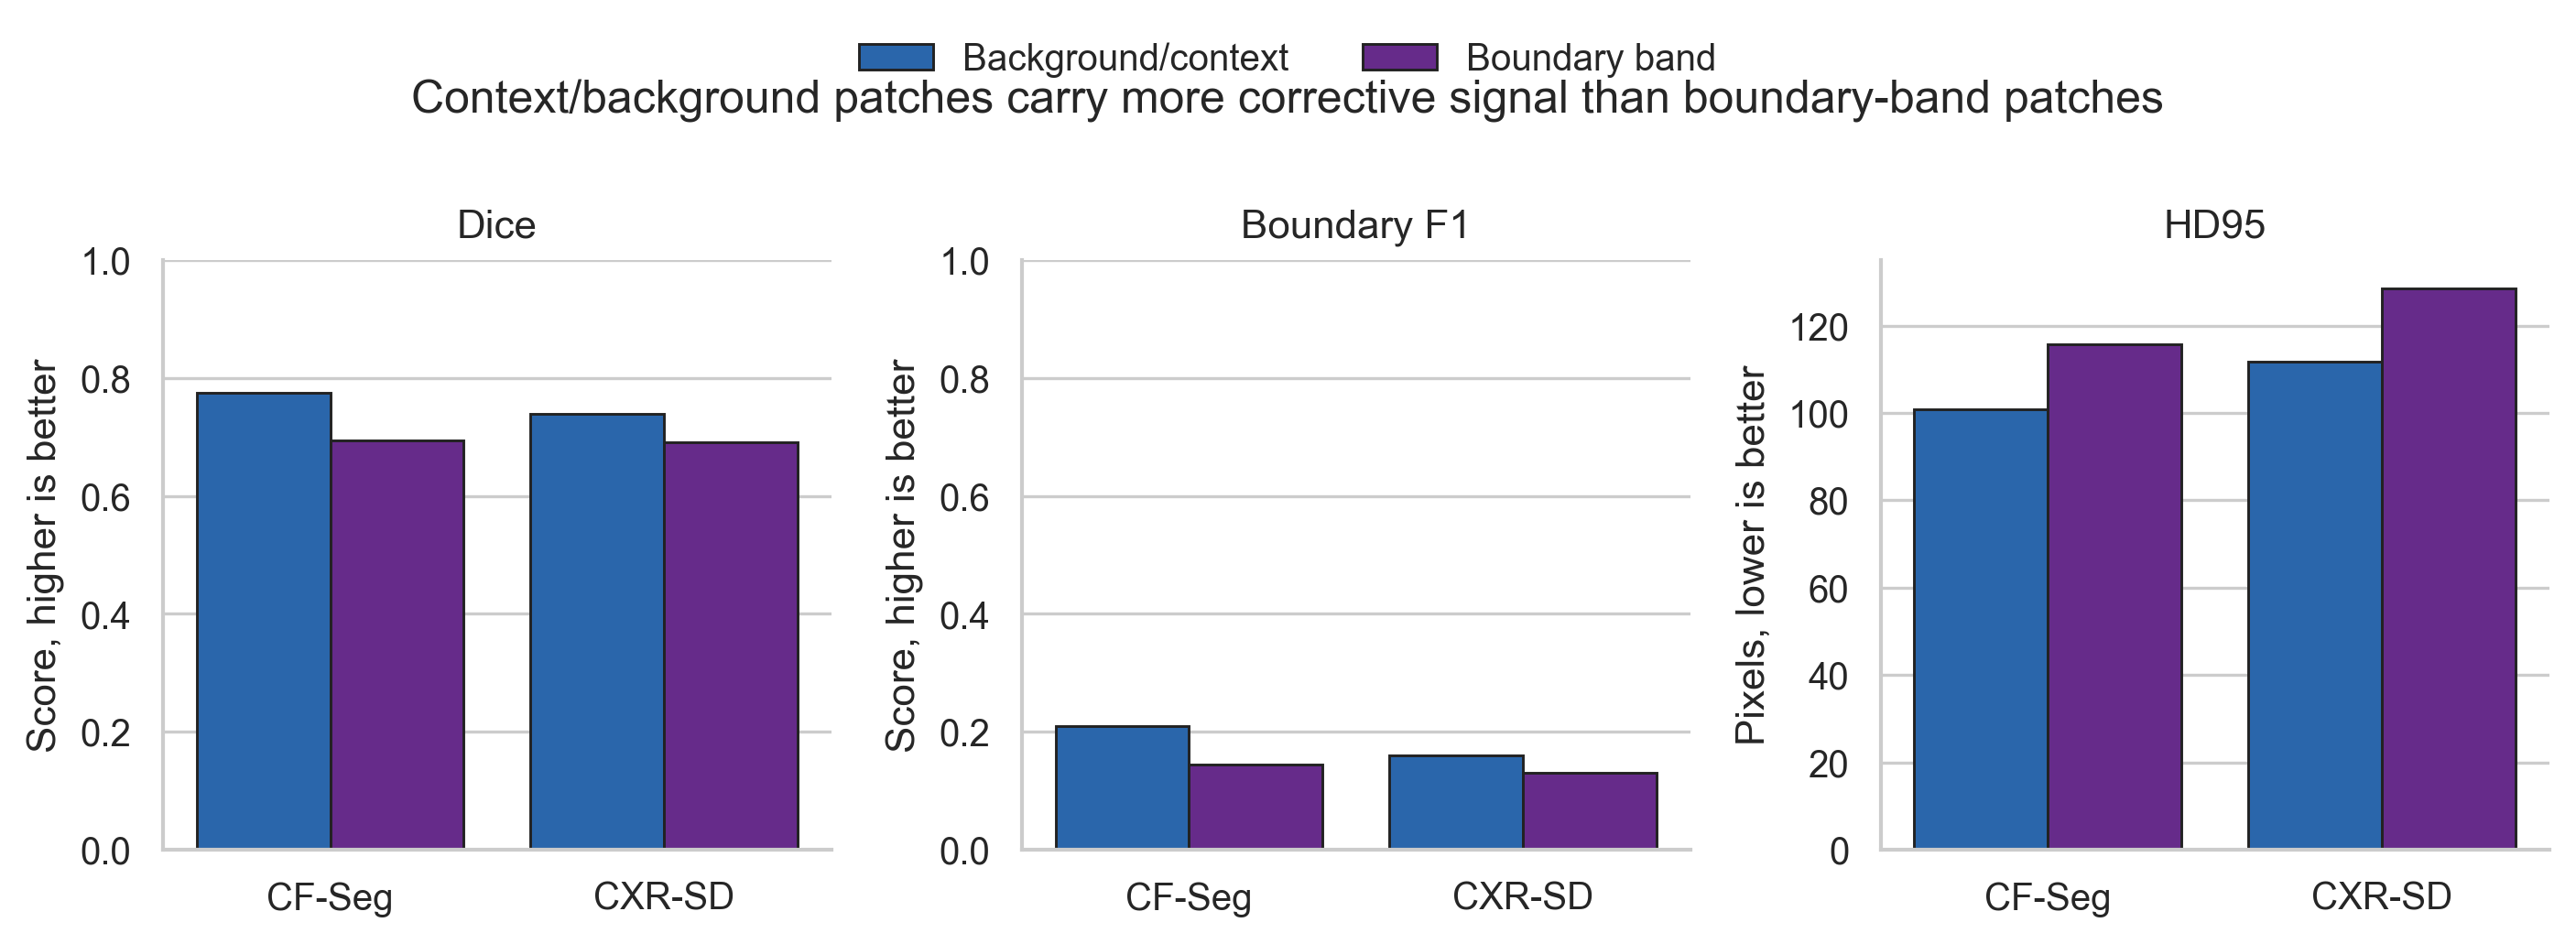
\includegraphics[width=0.92\textwidth]{figure_context_vs_boundary_controls.png}
\caption{Region controls. Background/context interventions carry more corrective signal than thin boundary-band interventions for both CF-Seg and CXR-SD counterfactuals. The failure manifests at the lung boundary, but the internal mechanism is more consistent with context-mediated shape correction than with a purely local boundary-token mechanism.}
\label{fig:regions}
\end{figure}

\subsection{Exploratory Failure Monitoring}

As an exploratory monitoring check, we used counterfactual activation-difference summaries to predict low-Dice MedSAM cases in the 50-case cohort. A balanced logistic regression with repeated stratified 5-fold cross-validation achieved ROC-AUC 0.730 using activation-difference features alone, compared with 0.749 for simple output-shape features and 0.771 when both were combined. Boundary-specific failure labels based on low Boundary F1 or high HD95 were better predicted by output-shape features in this small cohort. We therefore treat activation-based monitoring as a secondary observation: internal counterfactual features contain useful signal, but the stronger contribution of this paper is the causal patching evidence.

\section{Discussion}

The main result is that pseudo-healthy counterfactuals can serve as causal probes of a medical foundation model. CF-Seg counterfactuals improve MedSAM lung segmentation in pleural-effusion images, but the more important observation is internal: transplanting matched counterfactual activations into the diseased-image run reproduces the counterfactual mask behavior, while reverse and non-matched controls do not. This is a stronger mechanistic statement than saying that counterfactual preprocessing improves an output mask.

The region controls sharpen the interpretation. A natural hypothesis is that pleural-effusion failures are local boundary failures and therefore should be corrected by patching boundary-band activations. We find instead that broader background/context interventions carry more corrective signal. In chest radiography, the background outside a lung mask is not visually irrelevant; it contains pleural space, diaphragm position, lower thoracic context, and global shape cues. A context-mediated account is therefore plausible: MedSAM's boundary error may be driven by internal representations of thoracic layout and disease-obscured shape, not only by local edge evidence.

The diffusion experiments are deliberately conservative. CXR-SD improves Dice and HD95 but not Boundary F1 reliably, so it is not presented as a segmentation-quality winner. Its value is as a generator-diversity control: the matched-versus-non-matched activation-patching pattern and the context-over-boundary region pattern both persist when the counterfactual source changes. This reduces the chance that the mechanistic result is merely an artifact of one counterfactual generator.

\section{Limitations and Future Work}

The study uses a small 50-case cohort and CheXMask silver masks rather than expert lung-boundary annotations. CheXMask is appropriate for controlled workshop-scale mechanistic experiments, but it does not support clinical deployment claims. The analysis is also limited to lung segmentation under pleural effusion in NIH ChestX-ray14; additional pathologies, anatomies, modalities, and prompt types are needed to test generality. Finally, counterfactual images can introduce artifacts or alter patient-specific anatomy. Our matched, reverse, non-matched, and generator controls reduce this concern but do not eliminate it.

Future work should validate the mechanism with expert lung-boundary annotations, larger multi-source cohorts, and other anatomy/pathology pairs where disease changes the target boundary. A second direction is to move from activation patching to finer circuit analysis: identifying which attention blocks, channels, or token groups carry the context-mediated signal. A third direction is intervention design. If context activations reliably forecast or mediate failure, they could support inference-time monitoring, uncertainty flags, or targeted correction methods for medical segmentation foundation models.

\section{Conclusion}

Counterfactual activation patching reveals that MedSAM lung-boundary failures under pleural effusion are causally mediated by patient-specific internal image representations. Matched counterfactual activations restore counterfactual-quality segmentation, reverse patching restores original-like failure, and non-matched donors do not reproduce the effect. Spatial controls suggest that broader context and shape representations carry more corrective signal than a thin anatomical boundary band alone. These findings support counterfactual image pairs as practical mechanistic probes for medical foundation models, connecting internal model analysis to clinically meaningful failure modes.

\paragraph{Code Availability.}
An implementation and aggregate experiment outputs will be released publicly after review.

\begin{credits}
\subsubsection{\ackname}
Omitted for double-blind review.

\subsubsection{\discintname}
Competing-interest information is omitted for double-blind review and will be supplied in the submission system or camera-ready version.
\end{credits}

\begin{thebibliography}{16}

\bibitem{kirillov2023segment}
Kirillov, A., Mintun, E., Ravi, N., Mao, H., Rolland, C., Gustafson, L., Xiao, T., Whitehead, S., Berg, A.C., Lo, W.Y., Doll{\'a}r, P., Girshick, R.: Segment anything. In: Proceedings of the IEEE/CVF International Conference on Computer Vision (ICCV), pp. 4015--4026 (2023)

\bibitem{ma2024medsam}
Ma, J., He, Y., Li, F., Han, L., You, C., Wang, B.: Segment anything in medical images. Nature Communications \textbf{15}, 654 (2024)

\bibitem{mazurowski2023sam}
Mazurowski, M.A., Dong, H., Gu, H., Yang, J., Konz, N., Zhang, Y.: Segment anything model for medical image analysis: an experimental study. Medical Image Analysis \textbf{89}, 102918 (2023)

\bibitem{huang2024sammedical}
Huang, Y., Yang, X., Liu, L., Zhou, H., Chang, A., Zhou, X., Chen, R., Yu, J., Chen, J., Chen, C., Liu, S., Chi, H., Hu, X., Yue, K., Li, L., Grau, V., Fan, D.P., Dong, F., Ni, D.: Segment anything model for medical images? Medical Image Analysis \textbf{92}, 103061 (2024)

\bibitem{mehta2025cfseg}
Mehta, R., De Sousa Ribeiro, F., Xia, T., Roschewitz, M., Santhirasekaram, A., Marshall, D.C., Glocker, B.: CF-Seg: Counterfactuals meet segmentation. In: Medical Image Computing and Computer Assisted Intervention -- MICCAI 2025, LNCS, vol. 15967, pp. 117--127. Springer Nature Switzerland (2025)

\bibitem{rombach2022ldm}
Rombach, R., Blattmann, A., Lorenz, D., Esser, P., Ommer, B.: High-resolution image synthesis with latent diffusion models. In: Proceedings of the IEEE/CVF Conference on Computer Vision and Pattern Recognition (CVPR), pp. 10684--10695 (2022)

\bibitem{liang2023pie}
Liang, K., Cao, X., Liao, K.D., Gao, T., Ye, W., Chen, Z., Cao, J., Nama, T., Sun, J.: PIE: Simulating disease progression via progressive image editing. arXiv preprint arXiv:2309.11745 (2023)

\bibitem{wang2017chestxray8}
Wang, X., Peng, Y., Lu, L., Lu, Z., Bagheri, M., Summers, R.M.: ChestX-ray8: Hospital-scale chest X-ray database and benchmarks on weakly-supervised classification and localization of common thorax diseases. In: Proceedings of the IEEE Conference on Computer Vision and Pattern Recognition (CVPR), pp. 2097--2106 (2017)

\bibitem{gaggion2024chexmask}
Gaggion, N., Mosquera, C., Mansilla, L., Aineseder, M., Milone, D.H., Ferrante, E.: CheXmask: a large-scale dataset of anatomical segmentation masks for multi-center chest x-ray images. Scientific Data \textbf{11}, 511 (2024)

\bibitem{gaggion2025chexmask}
Gaggion, N., Mosquera, C., Aineseder, M., Mansilla, L., Milone, D., Ferrante, E.: CheXmask Database: a large-scale dataset of anatomical segmentation masks for chest x-ray images (version 1.0.0). PhysioNet (2025). \doi{10.13026/3705-zg36}

\bibitem{goldberger2000physionet}
Goldberger, A.L., Amaral, L.A.N., Glass, L., Hausdorff, J.M., Ivanov, P.C., Mark, R.G., Mietus, J.E., Moody, G.B., Peng, C.K., Stanley, H.E.: PhysioBank, PhysioToolkit, and PhysioNet: Components of a new research resource for complex physiologic signals. Circulation \textbf{101}(23), e215--e220 (2000)

\bibitem{vig2020causal}
Vig, J., Gehrmann, S., Belinkov, Y., Qian, S., Nevo, D., Sakenis, S., Huang, J., Singer, Y., Shieber, S.: Causal mediation analysis for interpreting neural NLP: The case of gender bias. In: Advances in Neural Information Processing Systems, vol. 33, pp. 9573--9585 (2020)

\bibitem{meng2022rome}
Meng, K., Bau, D., Andonian, A., Belinkov, Y.: Locating and editing factual associations in GPT. In: Advances in Neural Information Processing Systems, vol. 35, pp. 17359--17372 (2022)

\bibitem{zhang2023activationpatching}
Zhang, F., Nanda, N.: Towards best practices of activation patching in language models: metrics and methods. arXiv preprint arXiv:2309.16042 (2023)

\bibitem{imai2010causal}
Imai, K., Keele, L., Tingley, D.: A general approach to causal mediation analysis. Psychological Methods \textbf{15}(4), 309--334 (2010)

\bibitem{maierhein2024metrics}
Maier-Hein, L., Reinke, A., Godau, P., Tizabi, M.D., Buettner, F., Christodoulou, E., Glocker, B., Isensee, F., Kleesiek, J., Kozubek, M., Reyes, M., Riegler, M.A., Wiesenfarth, M., Baumgartner, M.: Metrics reloaded: recommendations for image analysis validation. Nature Methods \textbf{21}, 195--212 (2024)

\end{thebibliography}

\end{document}
